%%%%%%%%%%%%%%%%%%%%%%%%%%%%%%%%%%%%%%%%%%%%%%%%%%%%%%%%%%%%%%%%
%%%%%%%%%%%%%%%%%%%%%%%%%%%%%%%%%%%%%%%%%%%%%%%%%%%%%%%%%%%%%%%%
%%%%
%%%% This text file is part of the source of slides for
%%%% `The Art of HPC, vol 1: The Science of Computing'
%%%% by Victor Eijkhout, copyright 2012-2023
%%%%
%%%%%%%%%%%%%%%%%%%%%%%%%%%%%%%%%%%%%%%%%%%%%%%%%%%%%%%%%%%%%%%%
%%%%%%%%%%%%%%%%%%%%%%%%%%%%%%%%%%%%%%%%%%%%%%%%%%%%%%%%%%%%%%%%

\Level 1 {An informal introduction: the Game of Life}

\begin{frame}{Why}
  \begin{itemize}
  \item Parallelism has many aspects
  \item Let's look at a simple and structured problem
  \item Illustrate various aspects
  \end{itemize}
\end{frame}

\begin{frame}{Conway's Game of Life}
  \includegraphics[scale=.6]{life1}
\end{frame}

\begin{frame}{Conway's Game of Life}
  \includegraphics[scale=.4]{life2}

  \url{http://youtu.be/C2vgICfQawE?t=1m12s}
\end{frame}

\begin{frame}[fragile]{Code}
Evaluate $3\times3$ box:
\begin{verbatim}
def life_evaluation( cells ):
  # cells is a 3x3 array
  count = 0
  for i in [0,1,2]:
    for j in [0,1,2]:
      if i!=1 and j!=1:
        count += cells[i,j]
  return life_count_evaluation( cells[1,1],count )
\end{verbatim}
\end{frame}

\begin{frame}[fragile]{Code}
Naive implementation: save all boards
\begin{verbatim}
life_board.create(final_time,N,N)

for t in [0:final_time-1]:
  for i in [0:N-1]:
    for j in [0:N-1]:
      life_board[t+1,i,j] := 
        life_evaluation( life_board[t,i-1:i+1,j-1:j+1] )
\end{verbatim}
\end{frame}

\begin{frame}[fragile]{Code}
More efficient: just two boards
\begin{verbatim}
life_board.create(N,N)
temp_board.create(N,N)

for t in [0:final_time-1]:
  life_generation( life_board,temp_board )

def life_generation( board,tmp ):
  for i in [0:N-1]:
    for j in [0:N-1]:
      tmp[i,j] = board[i,j]
  for i in [0:N-1]:
    for j in [0:N-1]:
      board[i,j] = life_evaluation( tmp[i-1:i+1,j-1:j+1] )
\end{verbatim}
Can we do even better?
\end{frame}

\begin{frame}
  Parallelism: more than one processing element

  Parallel thinking: thinking about what can be done simultaneously,
  and what is really sequentially dependent.

  Example: Game of Life is three loops, inner two have conceptually
  independent iterations.

  (Strategy influences code design)
\end{frame}

\begin{frame}{Data parallelism}
  All cells are updated identically

  \includegraphics[scale=.1]{lifecollect}
\end{frame}

\begin{frame}{Data parallelism}
  Instruction level:

  \includegraphics[scale=.3]{simd}
\end{frame}

\begin{frame}[fragile]{Code transformation for data parallelism}
\small
\begin{columns}
\begin{column}{.45\hsize}
\begin{verbatim}
for i in [0:N]:
  for j in [0:N]:
    count = 0
    for ii in {-1,0,+1}:
      for jj in {-1,0,+1}:
        if ii!=0 and jj!=0:
          count += board[i+ii,j+jj]
\end{verbatim}
\end{column}
\begin{column}{.45\hsize}
\begin{verbatim}
for i in [0:N]:
  for j in [0:N]:
    count[j] = 0
  for ii in {-1,0,+1}:
    for jj in {-1,0,+1}:
      if ii!=0 and jj!=0:
        for j in [0:N]:
          count[j] += 
              board[i+ii,j+jj]
\end{verbatim}
\end{column}
\end{columns}

\end{frame}

\begin{frame}[fragile]{GPU data parallelism}
\begin{verbatim}
kerneldef life_step( board ):
    i = my_i_number()
    j = my_j_number()
    board[i,j] = life_evaluation( board[i-1:i+1,j-1:j+1] )

for t in [0:final_time]:
    <<N,N>>life_step( board )
\end{verbatim}
\end{frame}

\begin{frame}[fragile]{Loop-based parallelism}
OpenMP: instruction parallelism instead of data
\small
\begin{verbatim}
def life_generation( board,tmp ):
    # OMP parallel for
    for i in [0:N-1]:
        for j in [0:N-1]:
            tmp[i,j] = board[i,j]
    # OMP parallel for
    for i in [0:N-1]:
        for j in [0:N-1]:
            board[i,j] = life_evaluation( tmp[i-1:i+1,j-1:j+1] )
\end{verbatim}
(collapse nested loops)
\end{frame}

\begin{frame}{Coarse-grained parallelism}
  \begin{itemize}
  \item Data parallelism requires synchronization on instruction level
  \item Not possible for multicore and parallel processors
  \item $\Rightarrow$ coarser grained parallelism, for instance\\
    give each core/processor a subdomain of the Life board.
  \end{itemize}
\end{frame}

\begin{frame}{Work division}
  \includegraphics[scale=.1]{lifedivide}
\end{frame}

\begin{frame}{\ldots has some data implications}
  \includegraphics[scale=.1]{lifedivide-collect}

  Reads from neighbors, no conflicting writes
\end{frame}

\begin{frame}{Shared memory}
  \includegraphics[scale=.08]{shared}
\end{frame}

\begin{frame}{Distributed memory}
  \includegraphics[scale=.08]{distributed}

  Tricky: any remote data access has to be managed.
\end{frame}

\begin{frame}{Distributed memory in real life}
  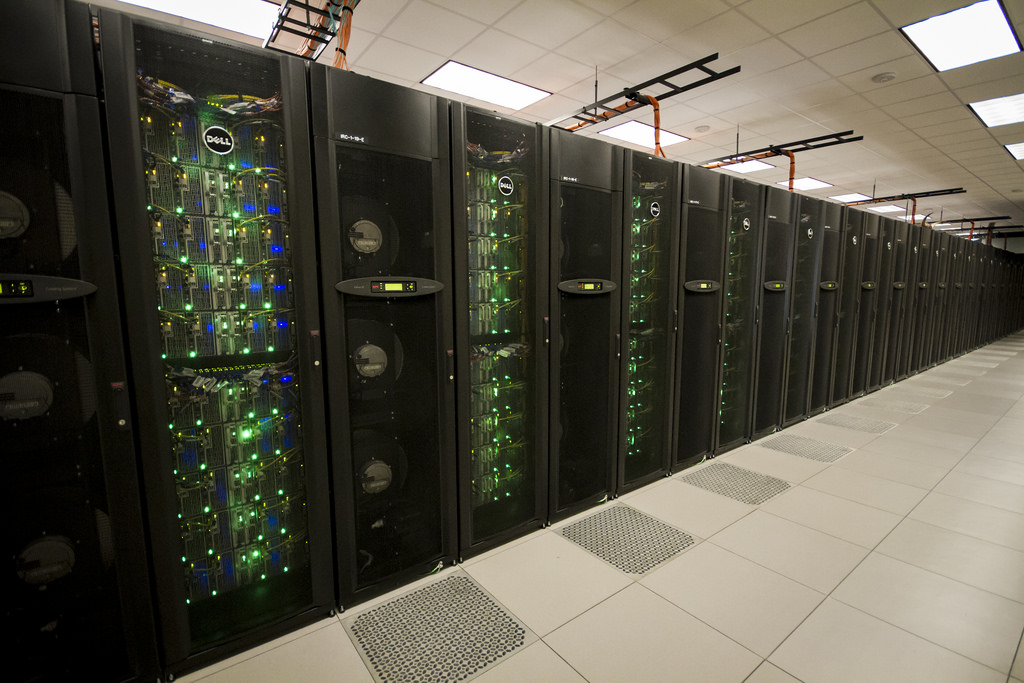
\includegraphics[scale=.25]{stampede-cable}
\end{frame}

\begin{frame}{\ldots takes a lot of cabling}
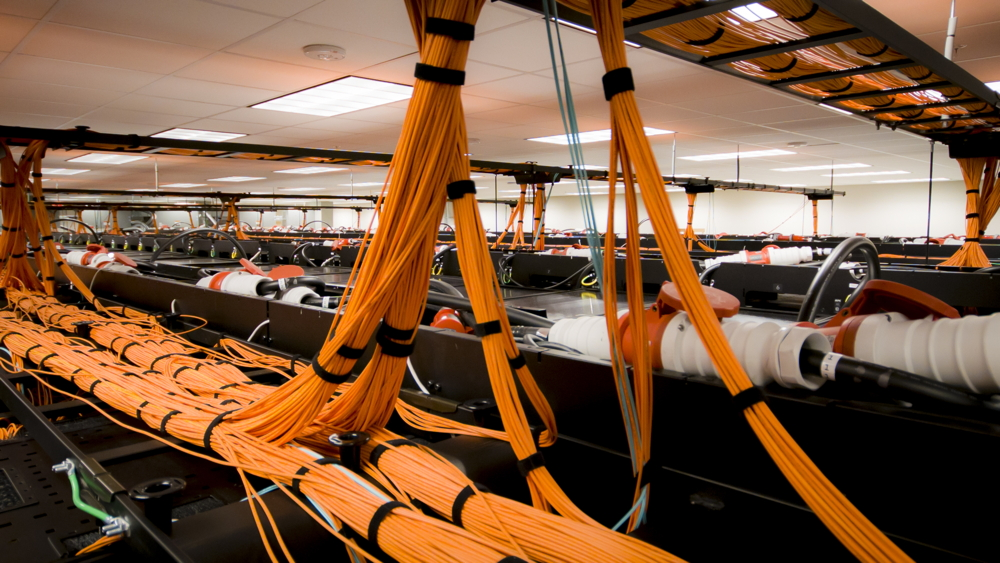
\includegraphics{stampede-overhead}
\end{frame}

\begin{frame}[fragile]{Message passing}
  \includegraphics[scale=.07]{mpiget}
\begin{verbatim}
high_line = MPI_Receive(from=p-1,cells=N)
low_line = MPI_Receive(from=p+1,cells=N)

tmp_line = my_line.copy()
my_line = life_line_update(high_line,tmp_line,low_line,N)
\end{verbatim}
\end{frame}

\begin{frame}{Task scheduling}
  \begin{itemize}
  \item So far: sequence of boards, parallelism in board
  \item Essential dependencies: $(i,j)$ depends on $(i\pm1,j\pm1)$,
  \item \ldots depends on $(i\pm2,j\pm2)$, and so on
  \end{itemize}
\end{frame}

\begin{frame}
\includegraphics[scale=.3]{life-tasks}
\end{frame}

\begin{frame}[fragile]{Declare tasks}
\begin{verbatim}
for t in [0:T]:
  for i in [0:N]:
    for j in [0:N]:
      task( id=[t+1,i,j], 
        prereqs=[ [t,i,j],[t,i-1,j],[t,i+1,j] # et cetera
                ] )
\end{verbatim}
\end{frame}

\begin{frame}[fragile]{Schedule tasks}
\begin{verbatim}
while there_are_tasks_left():
    for r in running_tasks:
        if r.finished():
            for t in scheduled_tasks:
                t.mark_available_input(r)
    t = find_available_task()
    p = find_available_processor()
    schedule(t,p)
\end{verbatim}
\end{frame}

\endinput

\begin{frame}[fragile]{Code}
\begin{verbatim}
\end{verbatim}
\end{frame}

\begin{frame}[fragile]{Code}
\begin{verbatim}
\end{verbatim}
\end{frame}

\begin{frame}[fragile]{Code}
\begin{verbatim}
\end{verbatim}
\end{frame}

\begin{frame}[fragile]{Code}
\begin{verbatim}
\end{verbatim}
\end{frame}
